%%% This Beamer example was created by LianTze Lim, April 2017.

%%%% This is a VERY simple and minimalistic beamer theme,
%%%% even reminiscent of marker pens on transparencies!
%%%% It mimics the look of the "seminar" package, which
%%%% can only be used with plain TeX.
%%%% There are also some comments and example to show how
%%%% to customise various elements, e.g. the font and colours.

\documentclass[11pt]{beamer}
%% If you'd like the default font size to be even larger, use 14pt or 17pt; these are supported by Beamer.

\graphicspath{{Figures/}{Figures}}

%%%%%%%%%%%%%%%%%%%%%%%%%%%%%%%%%%%%%%%%%
% These lines should usually go into a .sty file,
% but I'll leave them here so that it's easier to
% see how to customise a Beamer theme.
% Remember, the Beamer manual is your friend!!
% http://texdoc.net/pkg/beamer
%
%% So if your re-definitions have a @ somewhere, you
%% _MUST_ put a \makeatletter before these lines and then
%% \makeatother after them. This trick can only be done
%% in the preamble! BUT if you're doing these re-definitions
%% in a .sty file (so that you \usepackage it later), you
%% don't need the \makeatletter and \makeatother.
\makeatletter

%% Set the left and right margins
\setbeamersize{text margin left=1em,text margin right=1em}

%% FONTS
\setbeamerfont{title}{series=\bfseries,size=\LARGE}
\setbeamerfont{subtitle}{series=\bfseries,size=\Large}
\setbeamerfont{frametitle}{series=\bfseries,size=\small}
\setbeamerfont{block title}{series=\bfseries,size=\normalsize}
\setbeamerfont{footline}{size=\small}

%% COLOURS
%% If you'd like everything to have the same colour
\usebeamercolor{structure}
\setbeamercolor{normal text}{fg=structure.fg}

%% Add a line after the frametitle
\addtobeamertemplate{frametitle}{}{\vspace*{-1ex}\rule{\textwidth}{1pt}}

%% Use circular discs as itemized list markers;
%% there's an existing option in Beamer for it so I'll use it
\setbeamertemplate{itemize items}[circle]

%% Remove default navigation symbols (We'll add the ones we need in the footline
\setbeamertemplate{navigation symbols}{}


%% And before the footline... actually we'd like to re-define
%% the footline
\setbeamertemplate{footline}{%
   %% Beamer headlines and footlines are always full-paperwidth, so if you want the horizontal line to
   %% not span it entirely you'll need to do a bit of arithmetic
   \centering
   \begin{minipage}{\dimexpr\paperwidth-\beamer@leftmargin-\beamer@rightmargin\relax}
   \centering
   \rule{\linewidth}{1pt}\vskip2pt
   \usebeamerfont{footline}%
   \usebeamercolor{footline}%
   %% The frame number smack in the middle
   \hfill\insertframenumber/\inserttotalframenumber
   \hfill%
   %% ONLY the navigation symbols we want at the far right.
   %% We use an \llap so that it takes up zero width, and doesn't throw the page number off-centre!
   \llap{\insertframenavigationsymbol\insertbackfindforwardnavigationsymbol}\par
   \end{minipage}\vskip2pt
}

\setbeamercolor{block title alerted}{fg=white,bg=brown}

\makeatother
%%%% END STYLE CUSTOMISATION %%%%%%%%%%%%

\usepackage[english]{babel}
\usepackage[latin1]{inputenc}
\usepackage[T1]{fontenc}
\usepackage{graphicx}

\usepackage{subcaption}

\usepackage{times}

\usepackage{graphics}
%\usepackage[draft]{graphics}

\usepackage{xspace}
\usepackage{amsmath}
\usepackage{bm}
\usepackage{pgfpages}
\usepackage{fancybox}
\usepackage{threeparttable}
\usepackage{bbding}
\usepackage{verbatim}
\usepackage{booktabs}
\usepackage{fancyvrb}

\usepackage{natbib}
\bibpunct{(}{)}{;}{a}{}{,}

\newcommand{\pkg}[1]{{\normalfont\fontseries{b}\selectfont #1}}
\let\proglang=\textsf
\let\code=\texttt

\newcommand{\btheta}{ \mbox{\boldmath $\theta$}}
\newcommand{\bbeta}{ \mbox{\boldmath $\beta$}}
\newcommand{\balpha}{ \mbox{\boldmath $\alpha$}}
\newcommand{\by}{ \mbox{\bf y}}
\newcommand{\bY}{ \mbox{\bf Y}}
\newcommand{\bX}{ \mbox{\bf X}}
\newcommand{\bH}{ \mbox{\bf H}}
\newcommand{\bI}{ \mbox{\bf I}}
\newcommand{\bs}{ \mbox{\boldmath $s$}}

\title{Introduction to Coordinate Reference Systems}
\subtitle{}
\author{Bayesian modelling for spatial and spatio-temporal data}
\institute{MSc in Epidemiology}
\date{Week 6}


\begin{document}

\begin{frame}[t]
  \titlepage
\end{frame}


\begin{frame}
\frametitle{Coordinate Reference System (CRS)}
%https://datacarpentry.org/r-raster-vector-geospatial/09-vector-when-data-dont-line-up-crs/
\begin{itemize} \setlength\itemsep{\fill}
\item A coordinate system defines how the spatial elements of the data relate to the surface of the Earth.
\item The same CRS can often be referred to in many ways. In fact, each CRS is optimised to best represent the: (i) shape, and/or (ii) the distance and/or (iii) the area of features in a data set.
\item There is not a single CRS that does a great job at optimizing all three elements: shape, distance and area.
\end{itemize}
%refers to the way in which spatial data that represent the earth’s surface (which is round / 3 dimensional) are flattened so that you can “Draw” them on a 2-dimensional surface.
%http://resources.esri.com/help/9.3/arcgisengine/dotnet/89b720a5-7339-44b0-8b58-0f5bf2843393.htm
 %https://courses.washington.edu/gis250/lessons/projection/
\end{frame}


\begin{frame}
\frametitle{Types of CRS}
There are two main types of CRS:
\begin{itemize} \setlength\itemsep{\fill}
\item  \alert{Geographic coordinate systems (GCS)}: coordinate systems that identify any location on the Earth's surface using longitude and latitude, with units in decimal degrees or degrees.
\item \alert{Projected coordinate systems (PCS)}: coordinate systems that provide various mechanisms to project maps of the Earth's ellipsoid shape onto a two-dimensional Cartesian coordinate plan. They are localised to minimize visual distortion in a particular region. Examples are: Universal Transverse Mercator (UTM), Albers Equal Area, or Robinson, typically with units of feet or meters. Projected coordinate systems are referred to as \emph{map projections}.
\end{itemize}
\vspace{15pt}
%Coordinate systems (both geographic and projected) provide a framework for defining real-world locations.
%https://www.earthdatascience.org/courses/earth-analytics/spatial-data-r/geographic-vs-projected-coordinate-reference-systems-UTM/
\end{frame}

\begin{frame}
\frametitle{GCS \emph{vs} PCS}
\begin{figure}
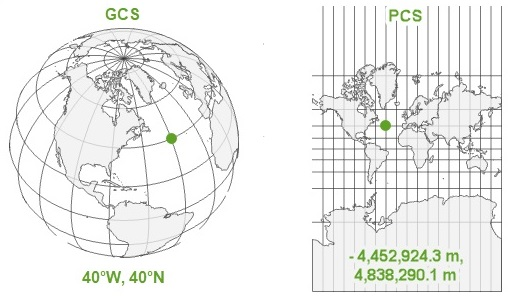
\includegraphics[width=9.5cm]{GCS_PCS.jpg}
\end{figure}
\tiny{Source: \url{https://www.esri.com/arcgis-blog/products/arcgis-pro/mapping/gcs_vs_pcs/}}
\end{frame}


\begin{frame}
\frametitle{Geographic coordinate systems [1]}
\small{A point is referenced by its longitude and latitude, which are angles measured from the Earth's center to a point on the Earth's surface.
%\vspace{-9pt}
\begin{itemize} %\setlength\itemsep{\fill}
  \item \emph{Longitude} is location in the East-West direction in angular distance from the Prime Meridian plane, %values are measured relative to the prime meridian and range from $-180^\circ$ when traveling west to $180^\circ$ when traveling east.; for most geographic coordinate systems, the prime meridian is the longitude that passes through Greenwich. Other countries use longitude lines that pass through Bern, Bogota, and Paris as prime meridians
  \item \emph{Latitude} is angular distance North or South of the equatorial plan. %values are measured relative to the equator and range from $-90^\circ$ at the South Pole to $+90^\circ$ at the North Pole.  A line of latitude is also known as a parallel.
\end{itemize}
}
\begin{figure}
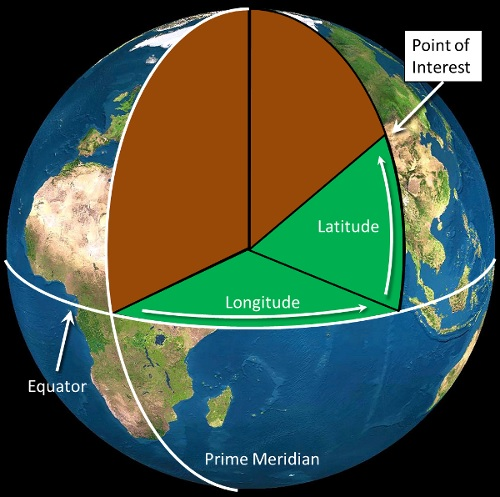
\includegraphics[scale=0.50]{GCS.jpg}
% latitude and longitude that specifies the angle between any point and the equator, and the angle between any point and the prime meridian.
%\tiny{\caption{The Earth represented as a globe with longitude and latitude values. Source: \url{http://gsp.humboldt.edu/OLM/Lessons/GIS/03%20Projections/IntroductionToCoordinateSystems1.html}.}}
\end{figure}
\tiny{Source: \url{http://gsp.humboldt.edu/OLM/Lessons/GIS/03\%20Projections/IntroductionToCoordinateSystems1.html}}
%https://desktop.arcgis.com/en/arcmap/latest/map/projections/about-geographic-coordinate-systems.htm
%https://geocompr.robinlovelace.net/spatial-class.html#crs-intro
%https://rspatial.org/raster/spatial/6-crs.html
\end{frame}



%\begin{frame}
%\frametitle{Geographic coordinate systems [II]}
%\begin{itemize} \setlength\itemsep{\fill}
%\item The surface of the Earth is represented by a \alert{spherical} or \alert{ellipsoidal} surface:
%\begin{itemize} \setlength\itemsep{\fill}
 % \item Spherical models are simple but are rarely used because they are inaccurate.
 % \item Ellipsoidal models are defined by two parameters: the equatorial radius and the polar radius. These are suitable because the Earth is compressed: the equatorial radius is around 11.5 km longer than the polar radius \citep{Lovelace2019}.
%\end{itemize}
%\end{itemize}
%https://geocompr.robinlovelace.net/spatial-class.html#crs-intro
%\end{frame}


\begin{frame}
\frametitle{Geographic coordinate systems [2]}
\begin{itemize} \setlength\itemsep{\fill}
  \item Obviously we cannot actually measure these angles, but we can estimate them. To do so, we need a model of the shape of the Earth. Such a model is called a \alert{datum}:
   \begin{itemize}\setlength\itemsep{\fill}
   \item it contains information on what \emph{ellipsoid} is used to approximate the Earth's shape and the relationship between the coordinate system and location on the Earth's surface; it also describes the origin $(0,0)$ of a coordinate system.
       \item There are two types of datum:
  \begin{itemize} \setlength\itemsep{\fill}
    \item \alert{local} such as NAD83 (North American Datum 1983) - the ellipsoidal surface is shifted to align with the surface at a particular location,%it fit very well in north America, but it will fit poorly in Australia where fit better GDA94
    \item \alert{geocentric} such as WGS84 (World Geodetic System 1984) - the center is the Earth's center of gravity and the accuracy of projections is not optimized for a specific location. It is used by the Global Positioning System (GPS).
        \end{itemize}
  \end{itemize}
\end{itemize}
%https://rspatial.org/raster/spatial/6-crs.html
%https://geocompr.robinlovelace.net/spatial-class.html#crs-intro
\end{frame}


\begin{frame}
\frametitle{Projected coordinate systems [1]}
\begin{itemize} \setlength\itemsep{\fill}
\item A major question in spatial analysis is how to transform this three-dimensional angular system to a two dimensional planar, sometimes called \alert{Cartesian} system.
%\item Projected CRSs are based on Cartesian coordinates on a flat surface.
\item The different types of planar coordinate reference systems are referred to as \alert{projections}.
%\item They have an origin, $x$ and $y$ axes, and a linear unit of measurement such as meters.
\item All projected CRSs are based on a geographic CRS and rely on map projections to convert the three-dimensional surface of the Earth into Easting and Northing (x and y) values in a projected CRS.
\item The transition leads to some distortions: there is not one best projection. Some projections can be used for a map of the whole world; other projections are appropriate for small areas only.
\end{itemize}
%https://geocompr.robinlovelace.net/spatial-class.html#crs-intro
%https://desktop.arcgis.com/en/arcmap/latest/map/projections/about-projected-coordinate-systems.htm
\end{frame}

\begin{frame}
\frametitle{Projected coordinate systems [2]}
There are three main projection types: conic, cylindrical, and planar:
\begin{figure}
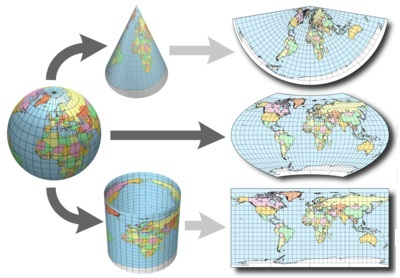
\includegraphics[scale=0.95]{Proj_CRS.jpg}
%{\tiny \caption{The 3-dimensional globe must be transformed to create a flat 2-dimensional map. Source: \url{https://www.earthdatascience.org/courses/earth-analytics/spatial-data-r/geographic-vs-projected-coordinate-reference-systems-UTM/}.}}
\end{figure}
\tiny{Source: \url{https://www.earthdatascience.org/courses/earth-analytics/spatial-data-r/geographic-vs-projected-coordinate-reference-systems-UTM/}}\\
%https://geocompr.robinlovelace.net/spatial-class.html#crs-intro
%https://desktop.arcgis.com/en/arcmap/latest/map/projections/about-projected-coordinate-systems.htm
\vspace{5pt}
\scriptsize A list of available projections can be found at \url{https://proj.org/operations/projections/}
\end{frame}

\begin{frame}
\frametitle{Differences in shape of United States boundaries associated with different projections}
\begin{figure}
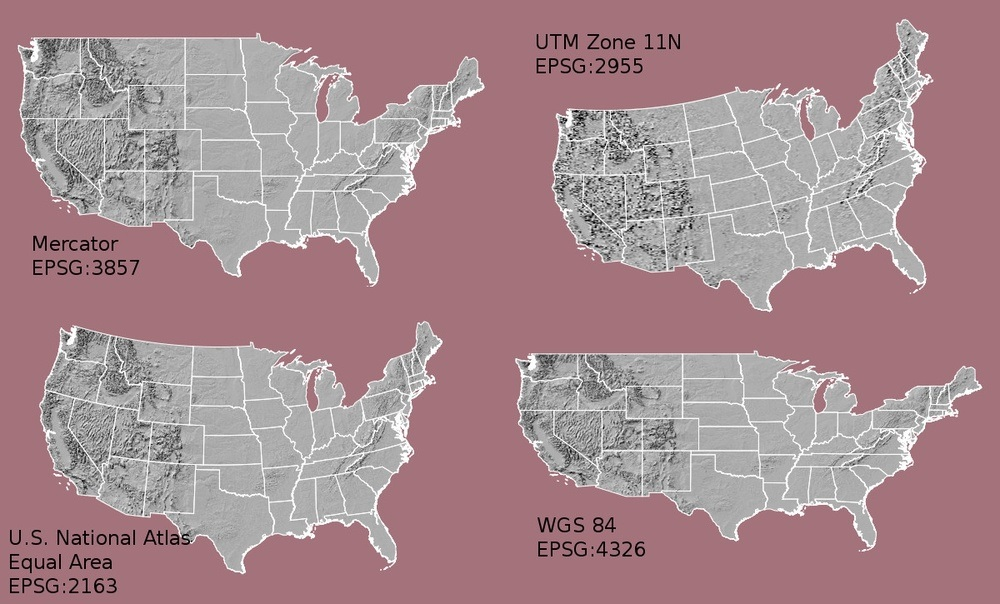
\includegraphics[scale=0.50]{US_CRS.jpg}
\end{figure}
\tiny{Source: Data Carpentry, \url{https://datacarpentry.org/r-raster-vector-geospatial/09-vector-when-data-dont-line-up-crs/}}.
\end{frame}

\begin{frame}
\frametitle{Re-projecting}
\begin{itemize} \setlength\itemsep{\fill}
\item Re-projecting is the process of changing the representation of locations from one CRS to another.
\item But when should data be transformed?
\begin{itemize} \setlength\itemsep{\fill}
\item The projections of locations on the Earth into a two-dimensional plane are \emph{distortions}, the projection that is best for an application may be different from the projection associated with the data we import. In these cases, data can be re-projected.
\item Another case is when two objects with different CRSs must be compared or combined. Thus, in the case of dealing with multiple data, re-projection permits to transform all data to a common CRS.
\end{itemize}
\item In R, to transform data to a different projection, we can use:
\begin{itemize}\setlength\itemsep{\fill}
  \item \texttt{spTransform()} function of the \texttt{rgdal} package
  \item \texttt{st\_transform()} function of the \texttt{sf} package
\end{itemize}
\end{itemize}
\end{frame}


\begin{frame} %[containsverbatim]
\frametitle{CRS in R (before 2020)}
\begin{itemize} \setlength\itemsep{\fill}
\item Spatial R packages support a wide range of CRSs and they use the \texttt{PROJ} library to perform conversions between cartographic projections. Before 2020, there are two ways of defining a CRS:
\vspace{3pt}
\begin{itemize} \setlength\itemsep{\fill}
\item via the  \texttt{\alert{proj4string}} definition, which specifies attributes such as the projection, the ellipsoid and the datum, for example the WGS84 longitude and latitude projection is specified as:
     {\scriptsize \color{green}$+proj=longlat +ellps=WGS84 +datum=WGS84 +no\_defs$}
     %syntax consists of a list of parameters, each prefixed with the +
     %String-based description of a coordinate reference system (CRS)
     \vspace{3pt}
\item the \texttt{\alert{EPSG}} numeric code (EPSG stands for European Petroleum Survey Group). The code refers to only one, well-defined coordinate reference system, for example the EPSG code of the WGS84 projection is 4326.
    %In R, using \texttt{sf} package:
\end{itemize}
\item Note that the EPSG code could not be available for a particular coordinate system. In R we can create a list of EPSG codes using the \texttt{make\_epsg()} function in \texttt{rgdal} package, or check online at \url{https://spatialreference.org/ref/epsg/}.
% but if a spatial object has a defined coordinate system, it will always have a \texttt{proj4} projection string.
%https://nowosad.github.io/whyr_webinar004/#21
\end{itemize}
\end{frame}

\begin{frame}
\frametitle{CRS in R (after 2020)}
There are new developments at level of \texttt{PROJ} (\url{https://proj.org/}), and shift from \texttt{proj4string} to the \texttt{OGC WKT2} representation (WKT stands for Well-known Text formats). Currently, in R:
%https://nowosad.github.io/whyr_webinar004/#22
\begin{itemize} \setlength\itemsep{\fill}
%\item Full support for ISO 19162:2018 WKT (also known as OGC WKT2)
\item The CRS is represented by a list with two components, \texttt{input} and \texttt{wkt}
% Open Geospatial Consortium (OGC)
% Well-known text representation of coordinate reference systems (WKT or WKT-CRS)
%\item Use \texttt{proj4string} is discouraged
\item Direct transformations from CRS to CRS (previously, the path was to transform first to WSG84 and from there to the target projection, increasing the risk of error between conversions)
\item Capability of time-dependent transformations (previously, static reference frames with no support for time-dependent datums, but on Earth, everything is moving, up to 80 mm/year)
%Using the \texttt{sf}, we can retrieve the CRS of an object using \texttt{st\_crs()}.
\end{itemize}
\end{frame}

\begin{frame}[containsverbatim]
\scriptsize{
%\begin{exampleblock}{}
\begin{semiverbatim}
library(spData)
library(sf)

# Extract the CRS information from the sf object nz (New Zealand)
st\_crs(nz) # here EPSG:2193

# Re-project 
nz_wgs <- st\_transform(nz, 4326) 
st\_crs(nz\_wgs) # now EPSG:4326

# Extract the CRS information from the sf object world
st\_crs(world) #EPSG:4326

# Re-project using the CRS of the sf object world
nz\_wgs = st\_transform(nz, st\_crs(world))
st\_crs(nz\_wgs)

# Remove the CRS from nz_wgs and plot the result
nz\_wgs\_NULL\_crs = st\_set\_crs(nz\_wgs, NA)

# Plots
par(mfrow = c(1, 3))
plot(st\_geometry(nz))
plot(st\_geometry(nz\_wgs))
plot(st\_geometry(nz\_wgs_NULL\_crs))

\end{semiverbatim}
%\end{exampleblock}
}
%https://geocompr.github.io/geocompkg/articles/solutions06.html
% what is wrong with this map of New Zealand and why?
%# answer: it is fatter in the East-West direction
%# because New Zealand is close to the South Pole and meridians converge there
% also https://rdrr.io/github/Robinlovelace/geocompr/src/code/chapters/06-reproj.R
\end{frame}

\begin{frame}
\begin{figure}
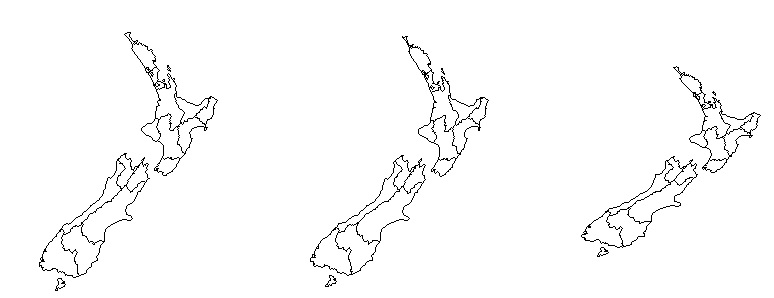
\includegraphics[scale=0.8]{NZ.jpg}
\end{figure}
\end{frame}



\begin{frame}

\begin{itemize} \setlength\itemsep{\fill}

\item For more details on CRS, see section $2.4$ and chapter 6 of Lovelace, R., Nowosad, J., and Muenchow, J. (2019), Geocomputation with R, CRC Press; the online version of the book is at \url{http://geocompr.robinlovelace.net/}
\item For  more details on new developments linked to PROJ, you can visit the links:
\url{https://proj.org/news.html}, and \url{https://info.crunchydata.com/blog/waiting-for-postgis-3-st_transform-and-proj6}  and \url{http://rgdal.r-forge.r-project.org/articles/PROJ6_GDAL3.html}
\end{itemize}
\end{frame}


%\begin{frame}[fragile]
%\citet{Lovelace2019} (Section 6.3) provide a useful function to calculate the EPSG code associated with any point on the planet:
%{\scriptsize
%\begin{exampleblock}{}
%\begin{verbatim}
%lonlat2UTM = function(lonlat) {
%  utm = (floor((lonlat[1] + 180) / 6) %% 60) + 1
%  if(lonlat[2] > 0) {
%    utm + 32600
%  } else{
%    utm + 32700
 % }
%}
%\end{verbatim}
%\end{exampleblock}
%}
%Thus, using London as an example, we can identify the UTM zone and associated EPSG code:
%{\scriptsize
%\begin{exampleblock}{}
%\begin{verbatim}
%library(sf)

%london = data.frame(lon = -0.1, lat = 51.5) %>%
%  st_as_sf(coords = c("lon", "lat")) # convert sp to sf object
%st_is_longlat(london)

%epsg_utm_lnd = lonlat2UTM(st_coordinates(london))

%st_crs(epsg_utm_lnd)$proj4string
%#[1] "+proj=utm +zone=30 +datum=WGS84 +units=m +no_defs"
%\end{verbatim}
%\end{exampleblock}
%}
%# we see the projection (+proj=utm), the zone (+zone=30) and units (+units=m)
%\end{frame}






\end{document} 